\section{Feature evaluation} \label{sec:body_feature_evaluation}

Concluding chapter \ref{sec:body_relevant_features} I have identified the following features that describe effective mnemonics. 
\begin{enumerate}
    \item word vividness (imageability, concreteness)
    \item bizarreness of mental imagery
    \item centrality of input words with strong connections in the output
\end{enumerate}

\subsection{Word vividness}
\textbf{Word norms}: Given the existing research it is plausible to start with quantifying the vividness of the mnemonics. It would be perhaps ideal to train a model that outputs a score that captures the vividness of the input text. Unfortunately I was unable to find such data. In the field of psycho-linguistics however norms of words exist. Several datasets are available that incorporate human word scores for different norms. Norms relevant to my research are: imageability, concreteness and sensory modality. The latter seems useful as words that are strongly identified with different senses are likely to be very concrete and contribute to vivid imagery.

One limitation that quickly emerges is that these datasets tend to be rather small and using them on their own won't cover enough words to be used effectively. Several successful attempts have been made to extend these norm datasets by training models that identify features from word embeddings \cite{concr_embed_bert, img_concr_svm, fusing_ctx_embed_concr}.

\cite{concr_embed_bert} referred to research showing that concrete word embeddings tend to cluster with other concrete ones while abstract ones show the same general behavior. This is not surprising as embeddings from increasingly sophisticated models encode features of text extracted from enormous corpora.

I mostly copied the architecture described in their paper to fine-tune DistilBERT for the regression task of predicting a concreteness scalar $c \in [0,1]$. In addition to the generous dataset of 40000 human concreteness ratings \cite{40000_concr} I trained the model with another 60000 multi word expressions from \cite{60000_concr}. This allows me to evaluate phrases rather than just words of the mnemonics in terms of concreteness. The fine-tuned model achieved a Pearson correlation of $0.88$ with the test data. Ten percent of the dataset had been used for testing. While this result is good the models of the paper performed up to $0.92$ in correlation.This gap in performance could be explained by the additional dataset used on my part. I suspect that it becomes less trivial to assess concreteness adding multi-word expressions to the training data.

To support that point I have fine-tuned BERT as described in the paper with just using the 40000 word ratings. This model achieved a Pearson correlation of $0.918$ which is close enough to confirm their results.

On a side note I hypothesized that more recent multi-modal models like CLIP are perhaps better suited for the task of predicting concreteness as they learn embeddings from text combined with images. My idea is that more abstract terms are in a different embedding space than concrete ones because they tend to have less distinct images associated with them. The set of possible images for the word \emph{cow} is probably a lot smaller than for the word \emph{female}.

To investigate this I've compared CLIP with BERT on predicting word concreteness. Two models for each architecture had been trained. One that fine-tuned all weights while the other one froze all weights except for the regression head. The latter gives us an idea of how well the raw embeddings are at predicting concreteness. It may have been more appropriate to use imageability ratings for this comparison but since imageability and concreteness are related and the existing data for the latter is far more abundant, I chose to use concreteness ratings for this task. 

\begin{table}[ht]
\centering
\begin{tabular}{@{}lcc@{}}
\toprule
Model & Unfrozen Weights & Frozen Weights \\ \midrule
BERT           & 0.918                     & 0.752                   \\
CLIP           & 0.905                     & 0.800                   \\ \bottomrule
\end{tabular}
\caption{Pearson correlations for BERT and CLIP with unfrozen and frozen weights.}
\label{tab:clip_bert_comparison}
\end{table}
As expected (see Table \ref{tab:clip_bert_comparison}) the CLIP model with frozen weights outperformed the BERT version, however it strikes me as surprising that the opposite effect was observed in the case of fine-tuning all weights. This may be explained due to architecture differences and would require further research.

Two more DistilBERT models have been fine-tuned to predict imageability and sensory modality scores. The latter was trained with 1792 examples \cite{Juhasz2013} gathered from participants that where asked to rate the degree to which each word evoked a sensory experience. The MRC psycholinguistic database \cite{mrc} contains 4828 imageability ratings which I used to train the former model. The models used for evaluating mnemonics and their test results are displayed in Table \ref{tab:linguistic_features_pearsonr}.

\begin{table}[ht]
\centering
\begin{tabular}{@{}lc@{}}
\toprule
Models          & Pearson Correlation \\ \midrule
Concreteness             & 0.880                        \\
Sensory Modality         & 0.706                        \\
Imageability             & 0.875                        \\ \bottomrule
\end{tabular}
\caption{Pearson correlation coefficients for the fine-tuned DistilBERT models}
\label{tab:linguistic_features_pearsonr}
\end{table}
Given the small training dataset the model predicting sensory modality achieved a mere correlation of $0.706$. Nonetheless I deemed it useful enough for further investigations.

\textbf{Method:} Perhaps the most straightforward way to evaluate the mnemonics is to take the mean (Equation \ref{eq:token_mean}) of the word scores from the individual models.
\begin{equation} \label{eq:token_mean}
    s_{\text{mnemonic}} = \frac{1}{N}\sum_{w=1}^{N}\text{model}(w)
\end{equation}
The mnemonics were first tokenized where punctuation and numbers had been removed. Moreover, I considered only words that were not labeled as stopwords. The results for sensory modality, imageability and concreteness are shown in Tables \ref{tab:mean_std_ser}, \ref{tab:mean_std_img}, \ref{tab:mean_std_concr} and Figures \ref{figure:ser_mean_box_plot}, \ref{figure:img_mean_box_plot}, \ref{figure:concr_mean_box_plot} respectively.
\begin{table}[ht] 
\centering
\caption{Means and Standard Deviations for Sensory Modality}
\label{table:group_stats}
\begin{tabular}{lcc}
\toprule
Group & Mean & Standard Deviation \\
\midrule
GPT-2& $0.337$ & $0.043$ \\
GPT-3 (mnemonic) & $0.320$ & $0.055$ \\
GPT-3 (paragraph)& $0.351$ & $0.065$ \\
WaniKani & $0.347$ & $0.063$ \\
\bottomrule
\end{tabular}
\label{tab:mean_std_ser}
\end{table}

\begin{table}[ht] 
\centering
\caption{Means and Standard Deviations for Imageability}
\label{table:group_stats}
\begin{tabular}{lcc}
\toprule
Group & Mean & Standard Deviation \\
\midrule
GPT-2& $0.558$ & $0.043$ \\
GPT-3 (mnemonic) & $0.569$ & $0.054$ \\
GPT-3 (paragraph)& $0.583$ & $0.065$ \\
WaniKani & $0.582$ & $0.063$ \\
\bottomrule
\end{tabular}
\label{tab:mean_std_img}
\end{table}

\begin{table}[ht] 
\centering
\caption{Means and Standard Deviations for Concreteness}
\label{table:group_stats}
\begin{tabular}{lcc}
\toprule
Group & Mean & Standard Deviation \\
\midrule
GPT-2& $0.558$ & $0.043$ \\
GPT-3 (mnemonic) & $0.569$ & $0.054$ \\
GPT-3 (paragraph)& $0.583$ & $0.065$ \\
WaniKani & $0.582$ & $0.063$ \\
\bottomrule
\end{tabular}
\label{tab:mean_std_concr}
\end{table}

\begin{figure}
    \centering
    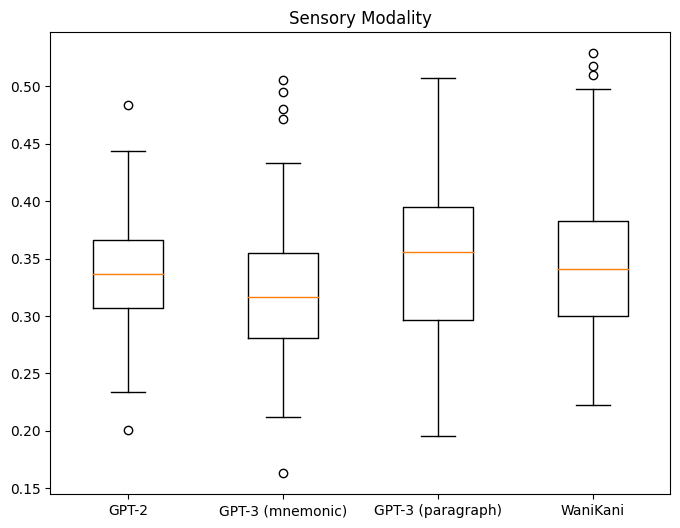
\includegraphics[width=400pt]{resources/ser_mean_box_plot.png}
    \caption{Sensory Modality Mean Scores}
    \label{figure:ser_mean_box_plot}
\end{figure}

\begin{figure}
    \centering
    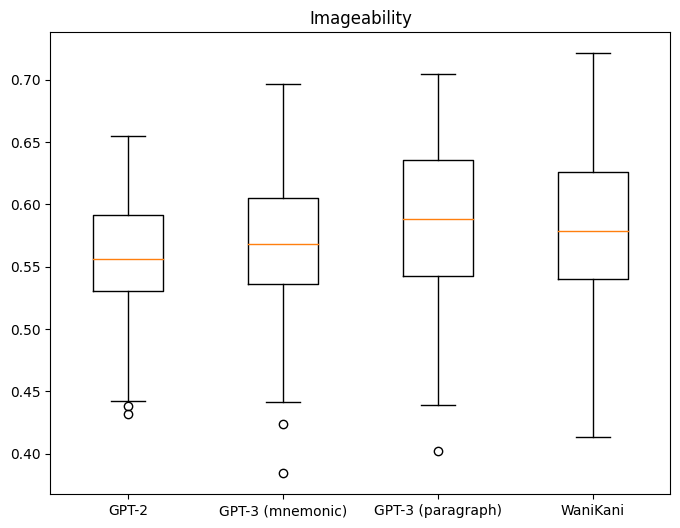
\includegraphics[width=400pt]{resources/img_mean_box_plot.png}
    \caption{Imageability Mean Scores}
    \label{figure:img_mean_box_plot}
\end{figure}

\begin{figure}
    \centering
    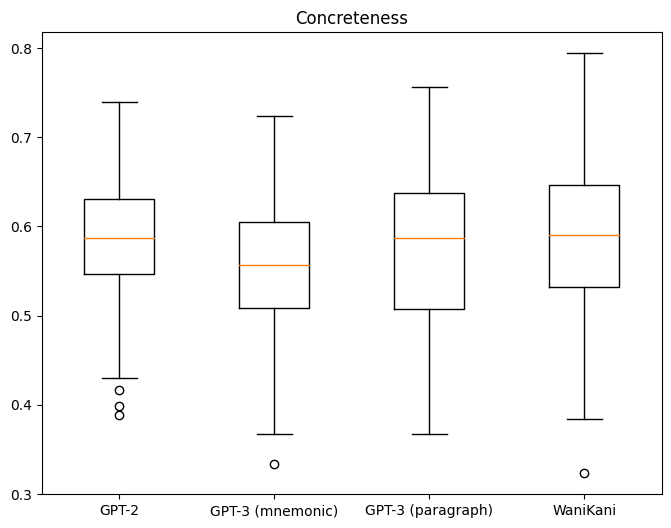
\includegraphics[width=400pt]{resources/concr_mean_box_plot.png}
    \caption{Concreteness Mean Scores}
    \label{figure:concr_mean_box_plot}
\end{figure}
\textbf{Discussion}: The ANOVAS's for all features were significant ($p < 0.05$). However, the differences are not very striking and the significant interaction terms between groups often show the opposite trend of what I had hoped for. Namely the paragraphs from GPT-3 often and GPT-2 generated mnemonics often have a higher overall mean than GPT-3 mnemonics and the WaniKani mnemonics.

I have also tried to use the $median$ and $maximum$ of mnemonic scores, but the results are comparable and therefore of no further interest. Given these results I conclude that simple metrics like $mean$, $median$, and $maximum$ of language norm scores over all tokenized words of individual mnemonics aren't very useful in separating the groups.
\subsection{Bizarreness}
Based on the observation that bizarre language uses words that are not commonly found together we may get some estimate of how bizarre a mnemonic is, based on the probability of their content occurring. To clarify this the phrase "a horse and a tiger racing each other" is probably a lot less likely to occur than seeing the phrase "two cars racing each other".

\textbf{Method}: To get a value for how likely text is to occur I will use perplexity scalars. This metric was explained earlier in Chapter \ref{sec:perplexity} (Equation \ref{eq:ppl}). One reason to be careful with this metric is that its measures are dependant on the training data and model architecture. For the experiment I used GPT-2 based perplexity which was trained with a dataset called WebText. This dataset was never fully published but contains mostly text from web pages that had been scraped by following outbound links from Reddit \cite{gpt2_hugging_face}. The results are shown in Table \ref{tab:ppl_whole_mnemonic} and plotted in Figure \ref{figure:ppl_whole_mnemonic}.     
\begin{table}[ht] 
\centering
\caption{Means and Standard Deviations for Perplexity}
\label{table:group_stats}
\begin{tabular}{lcc}
\toprule
Group & Mean & Standard Deviation \\
\midrule
GPT-2& $20.08$ & $12.71$ \\
GPT-3 (mnemonic) & $13.08$ & $4.30$ \\
GPT-3 (paragraph)& $22.63$ & $16.18$ \\
WaniKani & $36.13$ & $18.08$ \\
\bottomrule
\end{tabular}
\label{tab:ppl_whole_mnemonic}
\end{table}
\begin{figure}
    \centering
    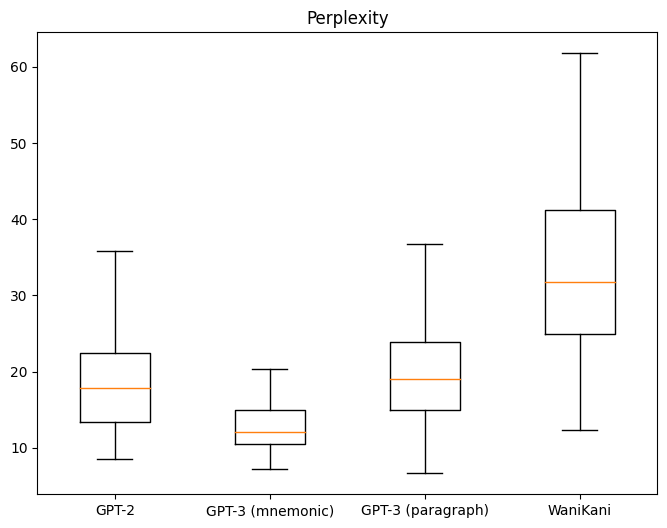
\includegraphics[width=400pt]{resources/ppl_entire_mnemonic.png}
    \caption{Perplexity Values}
    \label{figure:ppl_whole_mnemonic}
\end{figure}

\textbf{Discussion}: As is evident, the ANOVA was highly significant ($p = 0.000$). We can also observe the promising clear shift between WaniKani mnemonics and all other groups. The difference between the GPT-2 XL mnemonics and the WaniKani ones, however, is alarming. Given that the former frequently contains incoherent phrases due to the beam search constrains, I would have expected their perplexity values to be much higher.

Additionally the GPT-3 mnemonics have the overall lowest perplexity which renders the utility of perplexity for evaluating mnemonics questionable. The mnemonics by GPT-3 are storylike and often start with "Once upon a time". Perhaps the relatively low perplexity can be explained by taking a deeper look at the training data. It is possible that WebText contained a lot of story material. Moreover, the result may be explained by the model favoring output from other AI models over text written by humans. This poses an interesting question about the limitations of current language models that could be examined further. 
\subsection{Centrality}
One baseline requirement for any generation method was to include all input words in the generated mnemonic. While all groups fulfill this baseline, a quick look at the data reveals that the significance of the input words in the corresponding mnemonic varies a lot. In short good mnemonics revolve around the input words. I use the term \emph{centrality} to describe this phenomenon.

Given this insight it is plausible to utilize an exhaustive history of research on keyphrase extraction for the task of evaluating how central the input words are represented in the output. The idea is simple: input words should be keywords in mnemonics.

\textbf{Method}: Following I will benchmark four unsupervised keyword extraction algorithms for this task. I've come up with a recall based centrality score that leverages the scores for individual keyphrases.
\begin{equation}
    C(M, I) = \sum_{k \in E(M) \cap I} \frac{s(k)}{\sum_{k' \in E(M)} s(k')}
\end{equation}
The $E(M)$ represents the set of keyphrases extracted from the mnemonic. Only keyphrases that contain input words from $I$ are counted. They are weighted by the scores $s(k)$ given by the underlying extraction algorithm. These scores are then normalized.
YAKE and KPMiner are statistical models while TopicRank and MultipartiteRank are graph-based. Thanks to the \texttt{pke} \cite{pke} library the implementation of all algorithms is straightforward. The results are shown in Tables \ref{tab:yake_centrality}, \ref{tab:kpminer_centrality}, \ref{tab:topic_rank_centrality} and \ref{tab:multipartite_rank_centrality}.

\begin{table}[ht] 
\centering
\caption{Means and Standard Deviations for YAKE}
\label{table:group_stats}
\begin{tabular}{lcc}
\toprule
Group & M & SD\\
\midrule
GPT-2& $0.23$ & $0.22$ \\
GPT-3 (mnemonic) & $0.31$ & $0.18$ \\
GPT-3 (paragraph)& $0.32$ & $0.15$ \\
WaniKani & $0.40$ & $0.20$ \\
\bottomrule
\end{tabular}
\label{tab:yake_centrality}
\end{table}
\begin{table}[ht] 
\centering
\caption{Means and Standard Deviations for KPMiner}
\label{table:group_stats}
\begin{tabular}{lcc}
\toprule
Group & M & SD\\
\midrule
GPT-2& $0.31$ & $0.23$ \\
GPT-3 (mnemonic) & $0.42$ & $0.22$ \\
GPT-3 (paragraph)& $0.42$ & $0.21$ \\
WaniKani & $0.57$ & $0.22$ \\
\bottomrule
\end{tabular}
\label{tab:kpminer_centrality}
\end{table}
\begin{table}[ht] 
\centering
\caption{Means and Standard Deviations for TopicRank}
\begin{tabular}{lcc}
\toprule
Group & M & SD\\
\midrule
GPT-2& $0.15$ & $0.11$ \\
GPT-3 (mnemonic) & $0.33$ & $0.13$ \\
GPT-3 (paragraph)& $0.30$ & $0.13$ \\
WaniKani & $0.42$ & $0.14$ \\
\bottomrule
\end{tabular}
\label{tab:topic_rank_centrality}
\end{table}
\begin{table}[ht] 
\centering
\caption{Means and Standard Deviations for MultipartiteRank}
\begin{tabular}{lcc}
\toprule
Group & M & SD\\
\midrule
GPT-2& $0.15$ & $0.11$ \\
GPT-3 (mnemonic) & $0.35$ & $0.14$ \\
GPT-3 (paragraph)& $0.31$ & $0.14$ \\
WaniKani & $0.47$ & $0.15$ \\
\bottomrule
\end{tabular}
\label{tab:multipartite_rank_centrality}
\end{table}

\textbf{Discussion:} All ANOVAS's have been highly significant. As can be seen, all algorithms show a similar trend that is very promising. Overall the graph-based algorithms are slightly better and MultipartiteRank was the only one that had a significant interaction between GPT-3 mnemonics and paragraphs, favoring the former as expected. The best results are plotted in Figure \ref{figure:mpr_centrality}. I suspect that the statistical models are better suited for larger text samples as word frequency is an important feature for identifying keyphrases. The graph-based models are perhaps better at capturing the input words since graphs allow the models to represent semantic relationships between words and phrases. I hoped to quantify strong connections between input words. The graph, forming edges between nodes allows for that application.
\begin{figure}
    \centering
    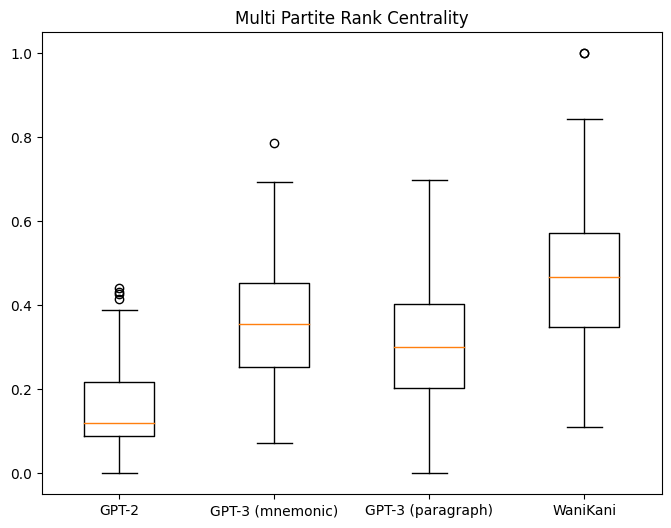
\includegraphics[width=400pt]{resources/mpr_centrality.png}
    \caption{MultipartiteRank Centrality Means}
    \label{figure:mpr_centrality}
\end{figure}

Given the success of matching the overlap of keywords and input words led me to question whether the word norms sensory modality, imageability and concreteness could significantly separate the groups if they were applied only to the keywords.

All of these tests had been statistically insignificant as well. However limiting the number of evaluated keywords to the length of the input words had a significant effect for concreteness and imageability. Despite this I decided to exclude their contribution to the final metric as the only way to get a perfect score would require the input word norms ratings to all equal 1.

Thus instead of getting an estimate of how imageable the mnemonic is, you would instead get a scalar that indicates how imageable the top $n$ keywords are, which ideally are the input words and therefore I'd simply rate the imageability of the input words.

Since the quality of the mnemonic should be independent of the input words I attempted to only score the imageability of the top $n$ keywords ($n = len(\text{input words})$) that do not include any input words. While these keywords may not include the input words, they could perhaps still be complementary to them and therefore be more vivid. This turned out to be insignificant as well.
\subsection{LLM Ranking}
Human feedback is expensive but necessary to further train large language models like the ones used in ChatGPT. Downstream, domain-specific tasks can fail because there are no labeled training data available. In these cases it is often unfeasible to gather the data with humans.

\cite{wang2021want} proposed to use GPT-3 in replacement of and in conjunction with human annotators to cut costs. They not only cut costs up to 96\% but also outperformed labels, fully ob humans, if GPT-3 labels were utilized together with human labels. The mixed method worked by using GPT-3's logits as confidence scores to decide when humans should step in to reannotate the labels. 

The success of LLMs to generate labels may question the utility of doing it in the first place, if the models can do the task already with few-shot learning. However the paper also concluded that training a task specific model with the generated labels outperformed the few-shot learning shortcut.

This research inspired me to test LLMs on their ability to rank order the mnemonics.

\textbf{Method:} I chose to use \texttt{gpt-3.5-turbo} for this task. The model was prompted with the task description followed by the four mnemonics.
\begin{description}
\item[Description]You are a human that rank orders mnemonics. The mnemonics have been constructed to help students learn Japanese Kanji and are based on its component meanings such that the Kanji meaning can be recalled easily. You are given four different mnemonics and you have to order them from most memorable to least memorable.
Output the ordered numbers separated by commas. E.g. 4,2,1,3 
\end{description}
Since the outputted data is ranked already I chose to do a Friedman test. It was highly significant. The means are shown in Table \ref{tab:gpt_ranks}.
\begin{table}[ht] 
\centering
\caption{Means for ChatGPT ranks}
\label{tab:gpt_ranks}
\begin{tabular}{lcc}
\toprule
Group & M \\
\midrule
GPT-2& $3.02$  \\
GPT-3 (mnemonic) & $1.01$ \\
GPT-3 (paragraph)& $3.12$ \\
WaniKani & $2.85$ \\
\bottomrule
\end{tabular}
\label{tab:multipartite_rank_centrality}
\end{table}

\textbf{Discussion:} The results show that on average the model favors GPT-3 and WaniKani mnemonics over the other two groups.

It is unexpected to see GPT-2 menmonics perform slightly better than the GPT-3 paragraphs given that they are often incoherent or fail to aim at the input words.

Overall GPT-3 mnemonics were always ranked first place except for one time. This may suggests a bias towards its own creation.

Most strikingly, WaniKani mnemonics did fairly bad. 30\% of the time they ranked 4th place. The advantage with these LLMs is that they can explain their decisions. E.g. when ranking WanKani last, the model explained itself like so: \emph{Mnemonic [4] connects the moon's power with the smell of one's armpit, which may not be the most appealing association.}. This example suggests that the model may reject the WaniKani mnemonics because of its reluctance to produce inappropriate or "unappealing" content.

In contrast, testing the same example with GPT-4, placed the WaniKani mnemonic on rank 3. This is the explanation it gave: \emph{This mnemonic takes a humorous approach, suggesting that the moon draws its power from the armpits of humans on Earth. The concept of "stinky power" being sapped from one's armpit creates a quirky image that can help with memorization.} Rather than rejecting this mnemonic because of its unappealing nature, GPT-4 values the "quirky image" it creates. This also suggests that the model understands inherent features of mnemonics very well as it highlights the vividness and bizarreness of the mnemonic. It would be interesting to see how GPT-4 compares to GPT-3 on the whole dataset. Unfortunately, at the time of this writing the API for the former is not available for me to use. 

These findings are very promising and may render simpler methods redundant as increasingly complex models like GPT-4 seem to have already a detailed understanding of the language used for mnemonics. While in \cite{wang2021want} the task specific models trained with generated labels still outperformed the "raw" models, the gap of performance will likely decrease with GPT-4 and there is no reason to suggest that this trend is not going to continue. Nonetheless, as of now, GPT-3 does not reliably separate the groups.
\subsection{Final Metric}
To conclude this chapter I propose a simplified metric that is essentially equivalent to \emph{recall}. Based on my previous findings (Figure \ref{figure:mpr_centrality} Multipartite Rank is used to extract keywords from the mnemonics and the score is simply the proportion of keywords that includes input words. Once an input word is found in the mnemonic it is only counted once. 
\begin{equation}
    S(K, I) = \frac{\sum_{i=1}^{|I|} 1(k_i \in I)}{|I|}
\end{equation}
This metric is closer to the initial hypothesis, namely, the set of $n$ top keywords should be the set of input words. It is also simpler as it does not depend on the weights of the underlying keyword extraction algorithm. Most importantly, it does a great job at separating the groups. The results are found in Table \ref{tab:final_metric_recall} and Figure \ref{figure:recall}.
\begin{table}[ht] 
\centering
\caption{Means and Standard Deviations for Recall}
\label{table:group_stats}
\begin{tabular}{lcc}
\toprule
Group & M & SD\\
\midrule
GPT-2& $0.18$ & $0.22$ \\
GPT-3 (mnemonic) & $0.51$ & $0.25$ \\
GPT-3 (paragraph)& $0.37$ & $0.24$ \\
WaniKani & $0.66$ & $0.26$ \\
\bottomrule
\end{tabular}
\label{tab:final_metric_recall}
\end{table}
\begin{figure}
    \centering
    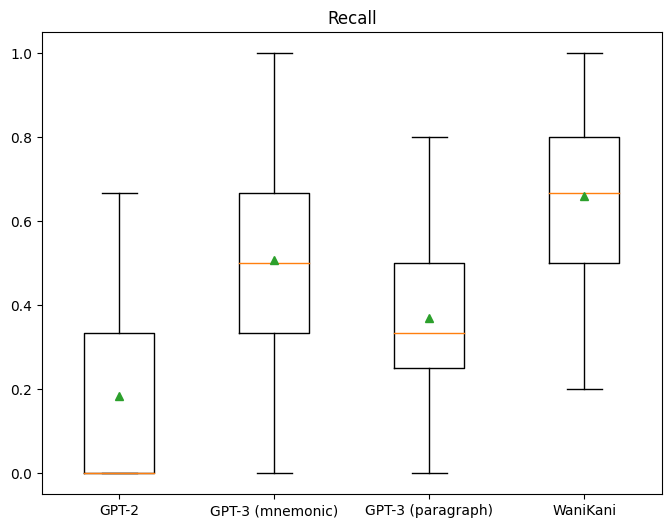
\includegraphics[width=400pt]{resources/recall.png}
    \caption{Recall}
    \label{figure:recall}
\end{figure}





